\documentclass{article}
% \usepackage[utf8]{inputenc} is no longer required (since 2018)

%Set the font (output) encoding
%--------------------------------------
\usepackage[T1]{fontenc} %Not needed by LuaLaTeX or XeLaTeX

%French-specific commands
%--------------------------------------
\usepackage[french]{babel}
\usepackage[autolanguage]{numprint} % for the \nombre command

%Hyphenation rules
%--------------------------------------
\usepackage{hyphenat}
\hyphenation{mate-mática recu-perar}
%--------------------------------------

% La première ligne charge le paquet, et la deuxième 
% ligne fixe la marge horizontale à 2,5 cm, et la marge verticale à 1,5 cm.
%--------------------------------------
\usepackage{geometry}
\geometry{hmargin=2.5cm,vmargin=1.5cm}
%--------------------------------------
% Pour inclure les images
\usepackage{graphicx}

\begin{document}
\tableofcontents

\vspace{1cm} %Add a 2cm space
\hspace{2cm}

\begin{abstract}
Ceci est un bref résumé du contenu du document écrit en français.
\end{abstract}

\section{Section d'introduction}
Il s'agit de la première section, nous ajoutons des éléments supplémentaires et tout sera correctement orthographiés. En outre, si un mot est trop long et doit être tronqué, babel va essayer de tronquer correctement en fonction de la langue.

\section{Réponses aux questions}

\subsection{Exercice 3}

1. On peut poser le graphe suivant : 


\begin{center}
    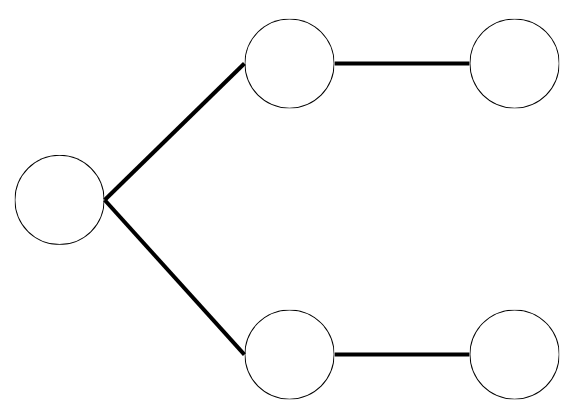
\includegraphics[scale=0.5]{Images/Ex3Q1Graphe1.png}
\end{center}

2. 

3.

\subsection{Exercice 4}

\subsubsection*{Partie 1}

\subsubsection*{Partie 2}
1. 


\subsubsection*{Partie 3}

3.

\subsubsection*{Partie 4}

\[ \lim x =  \theta + \nombre{152383.52} \]
\end{document}